\documentclass[conference]{IEEEtran}
\IEEEoverridecommandlockouts
\usepackage{cite}
\usepackage{amsmath,amssymb,amsfonts}
\usepackage{algorithmic}
\usepackage{graphicx}
\usepackage{textcomp}
\usepackage{xcolor}
\usepackage[brazilian]{babel}
\usepackage[utf8]{inputenc}
\usepackage[T1]{fontenc}
\def\BibTeX{{\rm B\kern-.05em{\sc i\kern-.025em b}\kern-.08em
    T\kern-.1667em\lower.7ex\hbox{E}\kern-.125emX}}
\begin{document}

\title{Perceptron de Multiplas camadas para Diagnóstico de Câncer de Mama}

\author{\IEEEauthorblockN{1\textsuperscript{o} Anara Olimpio}
    \IEEEauthorblockA{
        \textit{anaraolimpio@ig.com.br}
    }
    \and
    \IEEEauthorblockN{2\textsuperscript{o} Bruno Lopes}
    \IEEEauthorblockA{
        \textit{bruno.lopes.ti@icloud.com}
    }
    \and
}
\maketitle

\begin{abstract}
O câncer de mama é considerado o segundo tipo de câncer mais recorrente em mulheres, perdendo somente para o câncer de pele. De acordo com dados do Instituto Nacional do Câncer (INCA), em 2014, ocorreram mais de 57 mil casos de câncer de mama no Brasil em mulheres e, embora em quantidades bem pequenas, em homens. Diante do número alto de incidências, principalmente em mulheres, existe uma grande necessidade de pesquisa sobre o assunto. Este trabalho será baseado numa proposta de utilização de rede neural artificial para obter informações mais rápidas sobre o diagnóstico do câncer de mama utilizando como base para estudo e desenvolvimento do trabalho o conjunto de dados Breast Cancer Wisconsin. Este conjunto de dados de câncer de mama foi obtido do Hospital Universidade de Wisconsin, Madison, do Dr. William H. Wolberg. Os dados foram coletados, periodicamente, entre 1989 e 1991 com a ajuda do doutor Wolberg ao relatar seus casos clínicos o que possibilitou coletar as medidas dos tumores de mama. Os dados refletem uma ordem cronológico da coleta de dados e é um conjunto de dados de classificação. Há duas classes determinadas: benignas e malignas. Este conjunto de dados possui 699 registros e dimensão de 9 e baseado nessas informações pretendemos criar um padrão de comportamento que seja ágil em predizer se o tumor é maligno ou benigno.

\end{abstract}

\begin{IEEEkeywords}
Perceptron. Artificial Neural Network. Breast Cancer Wisconsin
\end{IEEEkeywords}

\section{INTRODUÇÃO}

\section{Referencial Teórico}
	%Problema, base conceitual para a solucao %
	
	Redes neurais artificiais (RNAs) são um modelos inspirados na arquitetura neural do cérebro e foi desenvolvido para tentar modelar a capacidade de aprendizagem de sistemas neurais biológicos \cite{b4}. Uma arquitetura típica de RNA conhecida como Perceptron de Multicamadas (MLP) contém uma série de camadas, compostas de neurônios e suas conexões. Um neurônio artificial tem a capacidade de calcular a soma ponderada de suas entradas e, em seguida, aplica uma função de ativação para obter um sinal que será transmitido para o próximo neurônio.
	
	O Modelo Perceptron foi desenvolvido nas décadas de 1950 e 1960 pelo cientista Frank Rosenblatt \cite{b9}, inspirado em trabalhos anteriores de Warren McCulloch e Walter Pitts. Hoje, é mais comum usar outros modelos de neurônios artificiais, mas o Perceptron permite uma compreensão clara de como funciona uma rede neural em termos matemáticos.
	
	Um Perceptron é um modelo matemático que recebe várias entradas, x1, x2, … e produz uma única saída binária:
	
	\begin{figure}[htbp]
	\centerline{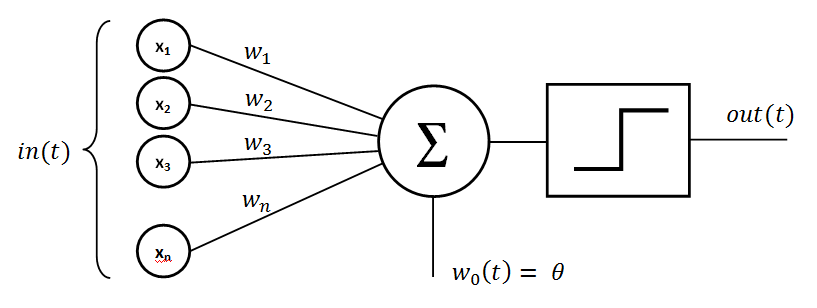
\includegraphics[scale=0.4]{Perceptron.png}}
	\caption{Fluxograma-Algoritmo PSO}
	\label{fig}
	\end{figure}
	
	No exemplo mostrado, o Perceptron possui três entradas: x1, x2, x3. Rosenblatt propôs uma regra simples para calcular a saída. Ele introduziu pesos, w1, w2, …, números reais expressando a importância das respectivas entradas para a saída. A saída do neurônio, 0 ou 1, é determinada pela soma ponderada, Σjwjxj, menor ou maior do que algum valor limiar (threshold). Assim como os pesos, o threshold é um número real que é um parâmetro do neurônio. Para colocá-lo em termos algébricos mais precisos:

Um Perceptron de multicamadas é uma variante do modelo Perceptron original proposto por Rosenblatt na década de 1950 \cite{b9}. Tem uma ou mais camadas escondidas entre suas camadas de entrada e saída, os neurônios são organizados em camadas, as conexões são sempre direcionadas de camadas inferiores para camadas, os neurônios na mesma camada não estão interligados.

Aprendizagem ou treinamento de RNA é equivalente a encontrar os valores de todos os pesos de tal forma que a saída desejada é gerada para correspondente entrada, pode ser visto como a minimização da função de erro computada pela diferença entre a saída da rede e o desejado na saída de um conjunto de observações de treinamento \cite{b6}.

Perceptron Multicamadas é o modelo muito utilizado em redes neurais artificiais que usando o back-propagation. A definição da arquitetura em redes MLP é um ponto muito relevante, a falta de conexões pode tornar a rede incapaz de resolver o problema de parâmetros ajustáveis, enquanto um excesso de conexões pode causar um ajuste excessivo dos dados de treinamento {b7}.



Um conjunto de dados para classificação de padrões consiste em vários padrões
juntamente com a sua classificação correta. Cada padrão consiste em um
número de medições (isto é, valores numéricos).
O objetivo consiste em gerar um classificador que tome as medidas
de um padrão como entrada e fornece sua classificação correta como saída. UMA
O tipo popular de classificador é o NN feed-forward [9].
Um NN feed-forward consiste de uma camada de entrada de neurônios, um
número de camadas ocultas e uma camada de saída. NNs feed-forward para
Os propósitos de classificação de padrões consistem em tantos neurônios de
padrões do conjunto de dados têm medições, ou seja, para cada medição
existe exatamente um neurônio de entrada. A camada de saída consiste em
muitos neurônios como o conjunto de dados tem classes. Dados os pesos de todos os
conexões de neurônios, a fim de classificar um padrão, um fornece sua
medições como entrada para os neurônios de entrada, propaga a saída
sinais de camada a camada até que os sinais de saída dos neurônios de saída
são obtidos. Cada neurônio de saída é identificado com um dos possíveis
classes. O neurônio de saída que produz o sinal de saída mais alto
classifica o respectivo padrão.



	
	\begin{figure}[htbp]
%	\centerline{\includegraphics[scale=0.4]{}}
	\caption{Fluxograma-Algoritmo PSO}
	\label{fig}
	\end{figure}
	
	
\section{Avaliação de Desenpenho}
    % Metodologia, experimentos e resultados, analise dos resultados(porques) %
  
\section{Resultado e Discussão}

   
    
\section*{Conclusão}

  

\begin{thebibliography}{00}

\bibitem{b1} AN EVOLUTIONARY ARTIFICIAL NEURAL NETWORK APPROACH FOR BREAST CANCER DIAGNOSIS. Washington: Third International Conference on Knowledge Discovery and Data Mining, 2010. Anual. ISBN: 9781424463979.

\bibitem{b2} Livraria digital do Instituto de Engenheiros Eletricistas e Eletrônicos (IEEE), AN EVOLUTIONARY ARTIFICIAL NEURAL NETWORK APPROACH FOR BREAST CANCER DIAGNOSIS, disponível em https://ieeexplore.ieee.org/document/5432472, acesso em 20 de setembro de 2018.

\bibitem{b3} Pfizer, industria farmacêutica, O câncer de mama em números no Brasil e no mundo, disponível em https://www.pfizer.com.br/noticias/Cancer-de-mama-em-numeros, acesso em 15 de setembro de 2018.

\bibitem{b8} UCI Machine Learning Repository, Breast Cancer Wisconsin, disponível em http://archive.ics.uci.edu/ml/datasets/Breast+Cancer+Wisconsin+(Original), acesso em 25 de agosto de 2018.

\bibitem{b4} Salchenberger LM, Cinar E, Lash NA. Neural networks: A new tool for predicting thrift failures. Decision Sciences. 1992;23(4):899–916

\bibitem{b5} Ramchoun H, Amine M, Idrissi J, Ghanou Y, Ettaouil M. Multilayer Perceptron: Architecture Optimization and Training. International Journal of Interactive Multimedia and Artificial Intelligence. 2016;4(1):26–30.

\bibitem {b6} M. Ettaouil and Y. Ghanou, “Neural architectures optimization and Genetic algorithms”, Wseas Transactions On Computer, Issue 3, Volume 8, 2009, pp. 526-537. 

\bibitem {b7} T.B Ludermir “Hybrid Optimization Algorithm for the Definition of MLP Neural Network Architectures and Weights” Proceedings of the Fifth International Conference on Hybrid Intelligent Systems (HIS’05) 0-7695- 2457-5/05 20.00 2005 IEEE.

\bibitem{b9} Rosenblatt, “The Perceptron: A Theory of Statistical Separability in Cognitive Systems”, Cornell Aeronautical Laboratory, Report No. VG1196-G-1, January, 1958. 

\end{thebibliography}
\end{document}

